\chapter{Theoretical Background}
In this chapter we give a introduction in various topics and areas which are necessary in order to understand the implementation of our pipeline and how its generated results were computed. 

\section{Optical Flow}
\label{sec:optical_flow}
In this section we explain the principles and the idea behind the optical flow. We emphasize this concept by giving an in intuitive definition, followed by a mathematical definition. Next, we discuss how such flow fields can be visualized. Lastly, we summarize and explain the pioneering formulation of HS used to estimate flow fields.

\subsection{Motion Example}
The optical flow is a visual phenomenon that describes the perception of motion.
By definition, it is the apparent visual motion a moving viewer experiences. \\ \\
To To give the reader a better, more intuitive understanding of this concept motion, have a look at figure $\ref{fig:motion_eg}$.
\begin{figure}[H]
\begin{center}
\subfigure[1st Frame]{
   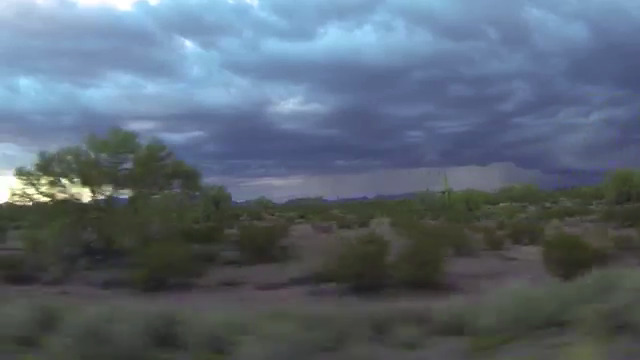
\includegraphics[width=0.47\linewidth] {background/of/ls1}
   \label{fig:motion_eg_f1}
}
\subfigure[2nd Frame]{
   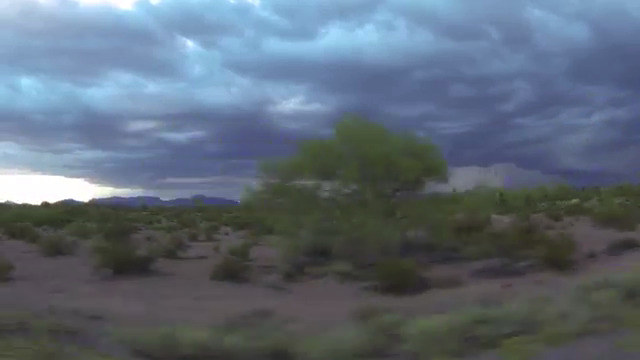
\includegraphics[width=0.47\linewidth] {background/of/ls2}
   \label{fig:motion_eg_f2}
}
~
\subfigure[3rd Frame]{
   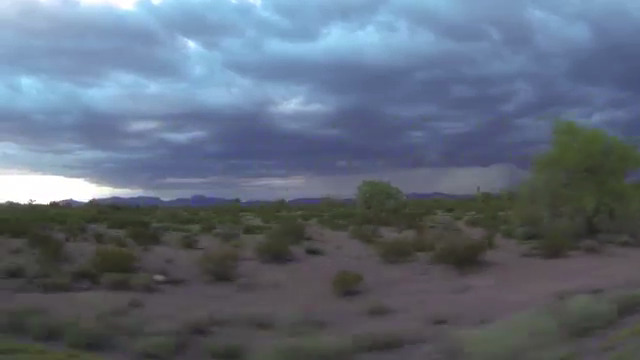
\includegraphics[width=0.47\linewidth] {background/of/ls3}
   \label{fig:motion_eg_f3}
}
\subfigure[4th Frame]{
   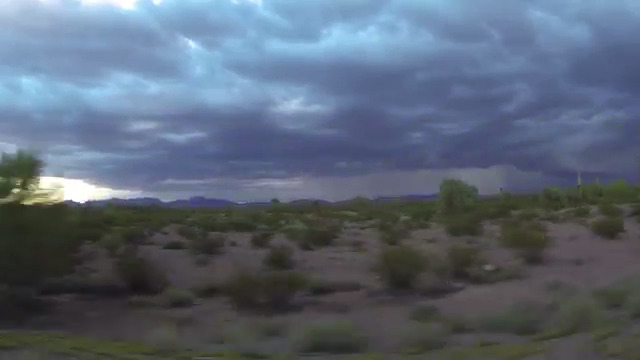
\includegraphics[width=0.47\linewidth] {background/of/ls4}
   \label{fig:motion_eg_f4}
}
\end{center}
\caption[Motion Example]{An example$\footnotemark$ of motion effects illustrated by four frames of a video sequence. Objects far away in the background, such as the mountain or the clouds seems to stand still. Objects being a fair distant apart, but also not too far away can be seen over several frames, such as the tree, that is passed. In addition, we also see observe, that the tree moves along the opposite direction as the driving car. Last, we also see the effect of motion blur for objects that are very close such as the grass.}
\label{fig:motion_eg}
\end{figure}
\footnotetext{The shown frames have been extracted from the following youtube video: \\ \url{https://www.youtube.com/watch?v=lo-pWLmMagc}}
Imagine you sit in a moving car and you are looking out of its windows. While doing so, you will observe that every overtaken object appear to move backwards. \\ \\
Furthermore, objects far in the background seem to stand still, whereas object close to the train seem to move very fast and thus have a blurry look. Therefore, the optical flow is an indicator for distance and size of an object. Moreover, the angle between the observer's viewing direction and the direction of the moving influences the optical flow. if an object travels perpendicular to the train or is directly above or below the it, then the optical flow is maximal. Lastly, an objects directly in front of a viewer will not exhibit any optical flow and thus appear to stand still. \\ \\
However, since not the whole object silhouette is directly in front of the viewer, its edges appear to move and therefore, the such an object appears to get either get larger or smaller, depending on its moving direction. \\ \\
In summary, the optical flow has the following key properties:
\begin{itemize}
  \item Overtaken objects appear to move backwards.
  \item Distant objects seem to move very slowly and close objects appear to move fast.
  \item The magnitude of the optical flow is doubles if either the speed of the traveling viewer is doubled or the distance to the observed object is halved.
  \item The optical flow varies depending on the angle between the viewing direction and and the direction of movement of the observed object.
  \item The optical flow is maximal if either the object is moving orthogonally towards the viewer's direction or it is moving directly above or below it.
  \item Objects directly in front of a viewer exhibit no optical flow.
\end{itemize}
The underlying basis input of our whole approach depicts the optical flow, computed from a given inputs sequence.

\subsection{Mathematical Formulation}
The optical flow ($\textbf{OF}$) is a vector field that defines a point-to-point correspondence between two successive frames. Each vector acts as the displacement of a point in the first frame to match its corresponding point in the second frame. In other words, the OF represents the pixel motion field as observed in images and thus answers the question which pixel went where in its successor frame. Ideally, the optical flow is the projection of the three dimensional motion on an image.\\ \\
The example in figure $\ref{fig:optical_flow_math_def_eg}$ visualizes this concept.
\begin{figure}[H]
\begin{center}
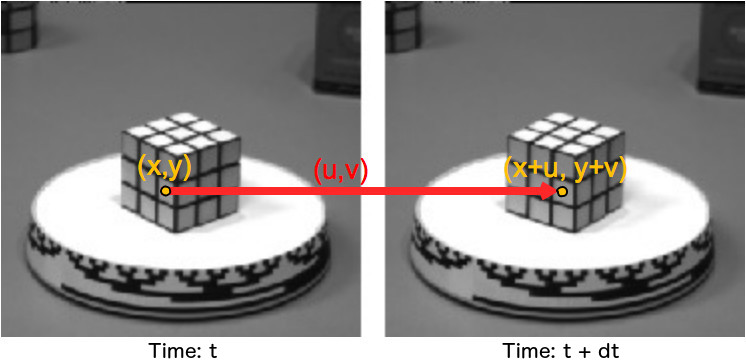
\includegraphics[width=1\linewidth] {background/of/rubiks_cube_frames}
\end{center}
\caption[Spinning Rubik's Cube]{An illustration$\footnotemark$ of two frames of a spinning Rubik's Cube. The point-to-point correspondence of s sample point (the orange point) is given by the optical flow, depicted as a red arrow.}
\label{fig:optical_flow_math_def_eg}
\end{figure}
\footnotetext{The unprocessed image shown in this figure has been taken from: \\ \url{http://robotics.eecs.berkeley.edu/~sastry/ee20/vision3/node2.html}}
In this figure two frames of a spinning Rubik's cube at different times are shown. The orange point $p = (x,y)$ at time $t$ is tracked to the position $(x+u, y+v)$ at time $t+dt$ by adding the optical flow $(u,v)$, visualized by a red arrow, to $p$. This matter of a fact can mathematically be modelled via the brightness consistency assumption, stated in equation $\ref{eq:of_brightness_const}$.
\begin{equation}
	I_{t} \left( x,y \right) = I_{t+dt} \left( x+u, y+v \right)
\label{eq:of_brightness_const}
\end{equation}
Where $I_t$ depticts the brightness at frame $t$.

\subsection{Visualization of Flowfields}
For visualizing flow fields we use the color encoding shown in subfigure $\ref{fig:color_encoding_flows_a}$. The shown color plate provides color values for the normalized flow vectors. The angle in the circle corresponds to the direction and the distance to the center to the velocity. \\ \\
Figure $\ref{fig:color_encoding_flows}$ also contains an example of a flow visualization using these color codes.
\begin{figure}[H]
\begin{center}
\subfigure[Flow Color Codes]{
   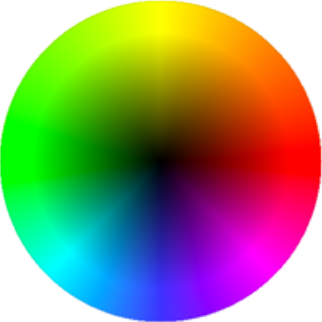
\includegraphics[width=0.35\linewidth] {background/of/flowfield_color_encoding}
   \label{fig:color_encoding_flows_a}
}
~
\subfigure[Example flow visualization]{
   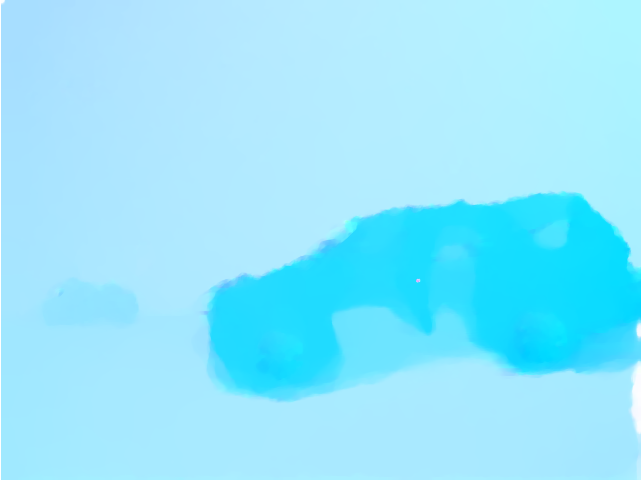
\includegraphics[width=0.5\linewidth] {background/of/cars_fwf_1}
   \label{fig:color_encoding_flows_b}
}
\end{center}
\caption[Visual Color Encoding of Flow Fields]{On the left a visualization of the color plate used to draw flow fields and on the right flow field visualized by this color scheme.}
\label{fig:color_encoding_flows}
\end{figure}

\subsection{Original Flow Estimation Method of H.S.}
\label{sec:hs_formulation}
In the pioneering work of $\cite{Hs81}$ B. Horn and B. Schnunck describe a technique to estimate the optical flow. Their method assumes smoothess in the flow over the whole image. Their flow estimation is formulated as a global energy functional and can numerically be solved via the Jocobi method$\footnote{The Jacobi method is an iterative method used to solve linear systems.}$. The advantage of their method is that it produces flows where the inner parts of homogeneous objects is filled in from the motion boundaries. However, its downside is that is is very sensitive to noise. \\ \\
Back then they defined the optical flow as the distribution of apparent velocities of movement of brightness patterns in an image. \\ \\
Moreover, they already understood the potential of the optical flow and stated the following properties: Can arise from relative motion of objects and the viewer and provide information about the spatial arrangement of the viewed objects and the rate of change in that arrangement. Discontinuities in the optical flow can help to perform segmentation tasks. \\ \\
Sticking to their flow definition they derived an equation that relates the change in the image brightness at a point to the motion of the brightness. \\ \\
Their formulation is based on the following assumptions:
\begin{itemize}
  \item The surface is assumed to be flat. This avoids brightness variations due to shading effects.
  \item The incident illumination is uniform across the surface. Then, the brightness at a point in the image is proportional to the reflectance of the surface at the corresponding point on the object.
  \item The Reflectance varies smoothly and has no spatial discontinuities. Having no discontinuities assures that the image brightness is differentiable.
  \item Situations where objects occlude one another are excluded.
\end{itemize}
These assumptions allow to conclude, that in their model the brightness of a particular point in the pattern is constant. \\ \\
Let the image brightness at a point $(x,y)$ in the image plane at time $t$ be denoted by $E(x,y,t)$. Since the brightness of any point is constant, $\frac{d E}{dt} = 0$ hold true. Using the chain rule for differentiation, they derived the expression in equation $\ref{eq:flow_eq}$.  
\begin{equation}
\begin{aligned}
0 &= \frac{d E}{dt} \\
&= \frac{\partial E}{\partial x} \frac{x}{dt} + \frac{\partial E}{\partial y} \frac{y}{dt} + \frac{\partial E}{\partial t} \\
&= E_{x} u + E_{y} v + E_{t}
\end{aligned}
\label{eq:flow_eq}	
\end{equation}
where we the following substitutions were used to derive the last identity of equation $\ref{eq:flow_eq}$:
\begin{equation}
\begin{aligned}
	u = \frac{dx}{dt} \text{ and } v = \frac{dy}{dt}
\end{aligned}
\end{equation}
By re-ordering the terms of equation $\ref{eq:flow_eq}$ the same way like it has been done in equation $\ref{eq:reordered_flow_eq}$:
\begin{equation}
\begin{aligned}
	(E_x, E_y) \cdot (u, v) &= -E_t \\
	\underbrace{-\frac{1}{E_t}\left( E_x, E_y \right)}_\text{known} \cdot \underbrace{(u, v)}_\text{unknown} &= 1
\end{aligned}
\label{eq:reordered_flow_eq}
\end{equation}
Hence, they could show that the change in image brightness can be formulated by a single linear equations with two unknowns $u$ and $v$, the so called $\textit{flow velocity}$. As a consequence, such a flow velocity cannot be computed locally without introducing additional constraints. \\ \\
In their formulation they express their additional constraint by stating that the square of the magnitude of the gradient of the optical flow velocity, as defined in equation $\ref{eq:smoothness_constraints}$, should be minimal.
\begin{equation}
	\left( \frac{\partial u}{\partial x} \right)^2 + \left( \frac{\partial u}{\partial y} \right)^2 \text{ and } \left( \frac{\partial v}{\partial x} \right)^2 + \left( \frac{\partial v}{\partial y} \right)^2
\label{eq:smoothness_constraints}
\end{equation}
The remaining problem then is to minimize the sum of the energies modelling the rate of image brightness change as stated in equation $\ref{eq:energy_brightness}$
\begin{equation}
	E_b = E_x u + E_y v + E_t
\label{eq:energy_brightness}
\end{equation}
and the measure of the departure from smoothness in the velocity flow, as formulated in equation $\ref{eq:energy_constraint}$.
\begin{equation}
	E_c^2 = \norm{\nabla u}^2 + \norm{\nabla v}^2
\label{eq:energy_constraint}
\end{equation}
The total error to be minimized is therefore equals to the energy term formulated in equation $\ref{eq:final_hs_energy_term}$.
\begin{equation}
	E = \int \int \left( E_b^2 + \alpha^2 E_c^2 \right) dx dy
\label{eq:final_hs_energy_term}
\end{equation}
This flow estimation formulation assumes smoothness in the flow over the whole image. Hence, minimzing this energy results in a minimization of distortions in the flow and thus prefers solutions which exhibit more smoothness. The scalar $\alpha$ acts as a regularization constant, that weights the influence of the smoothness term. Hence, larger values for $\alpha$ lead to soother flow estimations. \\ \\
This minimization can analytically be solved by formulating its multi-dimensional Euler-Lagrange equations as formulated in $\ref{eq:multi_dim_euler_lagrange}$.
\begin{equation}
\begin{aligned}
 \frac{\partial L}{\partial u} - \frac{\partial}{\partial x} \frac{\partial L}{\partial u_x} - \frac{\partial}{\partial y}\frac{\partial L}{\partial u_y} &= 0 \\
\frac{\partial L}{\partial v} - \frac{\partial}{\partial x} \frac{\partial L}{\partial v_x} - \frac{\partial}{\partial y}\frac{\partial L}{\partial v_y} &= 0  
\end{aligned}
\label{eq:multi_dim_euler_lagrange}
\end{equation}
where L denotes the integrand of the energy expression, given by equation $\ref{eq:def_l_euler_lag}$:
\begin{equation}
\begin{aligned}
E_x E_b - \alpha^2 \Delta u &= 0 \\
E_y E_b - \alpha^2 \Delta v &= 0 \\
\end{aligned}
\label{eq:def_l_euler_lag}
\end{equation}
Where $\Delta$ denotes the Laplace$\footnote{Definition of the Laplace operator in the two dimensional case: $\Delta = \frac{\partial^2}{\partial x^2} + \frac{\partial^2}{\partial y^2}$}$ operator.

When using a finite differences scheme for approximating the laplacian equation
as defined in equation $\ref{eq:finite_difference_laplacian}$
\begin{equation}
	\Delta u(x,y) = \bar{u} (x,y) - u(x,y)
\label{eq:finite_difference_laplacian}
\end{equation}
where $\bar{u} (x,y)$ denotes the weighted average of u computed by visiting the neighborhood around the pixel at location $(x,y)$, equation $\ref{eq:def_l_euler_lag}$ can be simplified to
\begin{equation}
\begin{aligned}
(E_x^2 + \alpha^2) u + E_x E_y v &= \alpha^2 \bar{u} - E_x E_t \\
(E_x^2 + \alpha^2) v + E_x E_y u &= \alpha^2 \bar{v} - E_y E_t
\end{aligned}
\label{eq:def_l_euler_lag_simplified}
\end{equation}
The equations in $\ref{eq:def_l_euler_lag_simplified}$ became linear in $u$ and $v$. This allows to solve this minimization problem for each pixel in the image. However, keep in mind that the solution depends on the neighboring values of the flow field. Hence, the system must be solved iteratively. The following update rule can therefore be used:
\begin{equation}
\begin{aligned}
 u_{k+1} &= \bar{u}_k - \frac{E_x (E_x \bar{u}_k + E_y \bar{v}_k + E_t)}{\alpha^2 + E_x^2 + E_y^2} \\
  v_{k+1} &= \bar{v}_k - \frac{E_y (E_x \bar{u}_k + E_y \bar{v}_k + E_t)}{\alpha^2 + E_x^2 + E_y^2}
\end{aligned}
\label{eq:hs_iteration}
\end{equation}

\section{General Motion Segmentation Pipeline}
%motion vectors are typically more homogeneous within an object region than color and texture. consequently, ambiguities in color baed segmentation disappear as soon as objects move.
%
%however, most objects do not move permanently (sometimes a moving object stops moving). moreover, articulated objects do not move homogeneously. deformation of body parts.
%=> causes severe problems in typical motion segmentation approaches based on two-frame optical flow.
In this section we describe a conceptually how the task of motion segmentation can be approached. \\ \\
In the following an ordered list of facts that determine our motion segmentation pipeline:
\begin{itemize}
  \item motion segmentation aims at decomposing a video in moving objects and into background by segmenting the objects that undergo different motion patterns.
  \item exploit long term aspect: motion is not considered independently for each frame but regard the whole motion history of a point to make a grouping decision.
  \item describe long-term motion of tracked points by a spatio-temporal curve called trajectory.
  \item point trajectories are an informative intermediate representation for the motion of object parts or whole objects.
  \item semi-dense point tracker based on optical flow that yields reliable trajectories for many frames.
  \item additionally, it increases the quality of the point tracking, especially at very fast moving regions
  \item all points showing some underlying structure are tracked until they are occluded. the occlusion reasoning is done based on the comparison of the forward and backward optical flow. when trajectroies get lost due to occlusion such that the sampling is sparser than the desidred rate, a new trajectory is started. the result is a set of reliable trajectories, that start in some frame of the sequence and end in another. depending on the data, many trajectories do not have any frame on common. However, the longer the are, the more useful motion information they are expected to carry.
  \item new problems arise: occlusion and disocclusion
  \item trajectories are usually asynchronous, i.e. they start and end in different frames.
  \item define a distance between all pairs of trajectories that share some common frames. 
  \item video segmentation approach: based on spectral clustering, where eigenvectors of the normalized graph laplacian are used to generate segmentations that approximate the optimal normalized cut.
\end{itemize}

\section{Data Clustering}
Clustering is a technique for exploratory data analysis and allows to identify groups of similar behaviour. 

\subsection{K-Means Clustering}
The idea of the k-means clustering algorithm is to partition $n$ observations into $k$ clusters in which each observation belongs to the cluster with the nearest mean. \\ \\
Given a set of observations $(\textbf{x}_1, \dots, \textbf{x}_n)$, where any $\textbf{x}_k \in \mathbb{R}^d$. k-means clustering tries to partition the $n$ observations into $k$ sets $\textbf{S} = \{ S_1, \dots, S_k\}$ to minimize the sum of distance functions of each point in the cluster to the $k$ centers. Mathematically, this can formulated as the follows:
\begin{equation}
	\argmin_{\textbf{S}} \sum_{i=1}^k \sum_{\textbf{x} \in S_i} \norm{\textbf{x} - {\boldsymbol {\mu }}_{i}}^2
\label{eq:k_means_minimzation_formulation}
\end{equation}
where ${\boldsymbol {\mu }}_{i}$ is the mean of points in $S_i$, the so called centroid. \\ \\
The k-means clustering equations $\ref{eq:k_means_minimzation_formulation}$ can be iteratively solved. Given an initial set of $k$ means $m_1^{(1)}, \dots, m_k^{(1)}$, the algorithm proceeds by alternating between two steps:
\begin{itemize}
\item \textbf{Assignment step}: Assign each observation to the cluster whose mean yields the least sum of distance functions of each point in the cluster. Since the sum of squares is the squared Euclidean distance, this is intuitively the "nearest" mean. 
\begin{equation}
  	S_i^{(t)} = \left\{ x_p \mid \forall j: 1 \leq j \leq k: \norm{x_p - m_i^{(t)}}^2 \leq \norm{x_p - m_j^{(t)}}^2 \right\}
\end{equation} 
where each $x_p$ is assigned to exactly one $S^{(t)}$.
\item \textbf{Update step}: Calculate the new means to be the centroids of the observations in the new clusters. 
\begin{equation}
	m_i^{(t+1)} = \frac{1}{\left| S_i^{(t)} \right| } \sum_{x_j \in S_i^{(t)}} x_j
\end{equation}
\end{itemize}
There are many initialization methods to assign the clusters such as randomly chooses k observations from the data set and uses these as the initial means or define k random clusters. The appropriate way of initializing the clusters depends on the given problem statement which the k-means attempts to address. 

\subsection{Graph Definitions}
In the following we offer the reader some basic graph definitions which are broadly used in this thesis. \\ \\ 
Let $G = (V, E)$ denote an undirected graph, where $V$ is the set of vertices and $E$ the set of edges. In this work we work with weighted graphs. This means that each edge between two vertices $v_i$ and $v_j$ has a non-negative weight $w_{ij}$. \\ \\
The $\textbf{weighted adjacency matrix}$ of the graph is the matrix 
\begin{equation}
W = \left( w_{ij} \right)_{i,j=1,\dots, n}	
\end{equation}
If $w_{ij} = 0$ then the vertices $v_i$ and $v_j$ are \textbf{not connected} by an edges. \\ \\
Since $G$ is supposed to be an \textbf{undirected graph}, we require
\begin{equation}
	\forall i,j : w_{ij} = w_{ji}
\end{equation}
The \textbf{degree} of a vertex $v_i \in V$ is defined as
\begin{equation}
	d_i = \sum_{j=1}^n w_{ij}
\end{equation}
In fact the sum accumulates only vertices that are adjacent to $v_i$, since all other vertices have a weight equals zero. \\ \\
The \textbf{degree matrix} $D$ is defined as the diagonal matrix with the degrees $d_1,\dots, d_n$ on the diagonal. \\ \\
For a given subset of vertices $A \subset V$, its \textbf{complement} is defined as
\begin{equation}
	\bar{A} = V \setminus A
\end{equation}
The \textbf{indicator function} is defined as
\begin{equation}
\begin{aligned}
& \mathbbm{1}_A = \left( f_1, \dots, f_n \right)^{T} \in \mathbb{R}^n \\
& \text{where } \forall i: f_i= 
\begin{cases}
    1,& \text{if } v_i\in A\\
    0,              & \text{otherwise}
\end{cases}
\end{aligned}
\end{equation}
For the set of indices $\{ i : v_i \in A \}$ we use the shorthand notation $i \in A$. For two subsets $A, B \subset V$, which are not necessarily disjoint, we define their \textbf{set sum} as
\begin{equation}
	W(A,B) = \sum_{i \in A, j \in B} w_{ij}
\end{equation}

\subsection{Similarity Graph}
Given a set of data points $x_1, \dots, x_n$ and some notion of similarity $s_ij \geq 0$ between all pairs of data points $x_i$ and $x_j$. Then, our goal is to divide the data points into several groups such that points in the same group are similar and points in different groups are dissimilar to each other. To address this task we represent our data by a similarity graph $G = (V, E)$. \\ \\
Each vertex $v_i$ in this graph represents a data point $x_i$. Two vertices are connected if the similarity $s_{ij}$ between the corresponding data point $x_i$ and $x_j$ is positive or larger than a certain threshold and the edge is weighted by $s_{ij}$. The data clustering problem becomes then to the graph partitioning problem. Find a partition of the graph such that the edges between different groups have very low weights$\footnote{This means that points in different clusters are dissimilar from each other.}$ and edges within a group have high weights$\footnote{which means that points within the same cluster are similar to each other}$. \\ \\
There are several constructions to transform a given set of data points with pairwise similarities $s_{ij}$ or pairwise distances $d_{ij}$ on the graph. The common goal of such a construction is to to model the local neighborhood relationships between the data points. In the following several a list of different construction types.
\begin{itemize}
	\item The \textbf{$\epsilon$-neighborhood graph}: All points whose pairwise distances are smaller than a given $\epsilon$ are connected. In that case the distances between connected vertices is at the same scale (at most equals $\epsilon$). Hence, the edge weights do not incorporate additional information about the data on the graph and thus, such a graph is usually considered as an unweighted graph.
	\item The \textbf{k-nearest neighbor graph}: Vertex $v_i$ is connected with $v_j$ if $v_j$ is among the k-nearest neighbors of $v_i$. This definition usually leads to a directed graph, since this neighborhood relationship is not symmetric. When interested in constructing a undirected graph, we can either ignore the induced edge directions (corresponds to an OR relationship) or connect the vertices if and only if both are nearest neighbors of each other (corresponds to an AND relationship).
	\item The \textbf{fully connected graph}: All points that exhibit a positive similarity are connected with each other. The edge weight corresponds to their similarity value.
\end{itemize}
For measuring the distances between data points several metrics can be used, such as the euclidean distance or other norms. However, when dealing with spectral clustering a prominent distance measure is the is the Gaussian similarity function
\begin{equation}
	s(x_i, x_j) = e^{\frac{-\norm{x_i - x_j}^2 }{2 \sigma^2}} 
\end{equation}
where $\sigma$ controlls the neighborhood width.

\subsection{Spectral Clustering}
%TODO: maybe we should introduce a section called filtering, containing bilateral filtering, harris corner detector and so forth..
Kernighan-Lin Heuristic, Graph Cut
multi-label CRF on superpixels for class segmentation $\cite{Fulkerson2009}$
$\cite{Ker70}$


\section{On Filtering Images}
\subsection{Gaussian Filter}

A Gaussian filter (\textbf{GF}) is a linear operator that reduces noise by smoothing the image. Applying GF corresponds to a low-pass filtering.
At each position it estimates a local average of the intensities as defined in equation $\ref{eq:gaussian_filtering_def}$.
\begin{equation}
	\mathcal{F}^{\text{gf}} \{I \} (p) = \sum_{q \in \Omega_p} G_{\sigma} (\norm{p - q}) I_q
\label{eq:gaussian_filtering_def}
\end{equation}
where $I$ defines the input image and $\Omega_p$ contains all neighboring points within the window that are centered at the image point $p$. Moreover, $G_{\sigma}$ denotes the two dimensional Gaussian kernel, which is defined in equation $\ref{eq:def_g_weight}$.
\begin{equation}
	G_{\sigma} (x) = \frac{1}{2 \pi \sigma^2} e^{-\frac{x^2}{2 \sigma^2}}
\label{eq:def_g_weight}
\end{equation}
The Gaussian filtering is the weighted average of the intensity of the adjacent positions with a weight decreasing with the spatial distance to the center position. This distance is defined by $G_{\sigma} (\norm{p - q})$ where $\sigma$ is a parameter that defines the size of the neighborhood. The resulting image is a blurred version of the input image.

\subsection{Bilateral Filter}
A Bilateral filter (\textbf{BF}) is a non-linear operator that reduces noise by smoothing the image but at the same time preserves its edges. \\ \\
The rational of this filter is that two pixels are close to each other if not only if their spacial distance is small but also if they are similar regarding their intensity range.
\begin{figure}[H]
\begin{center}
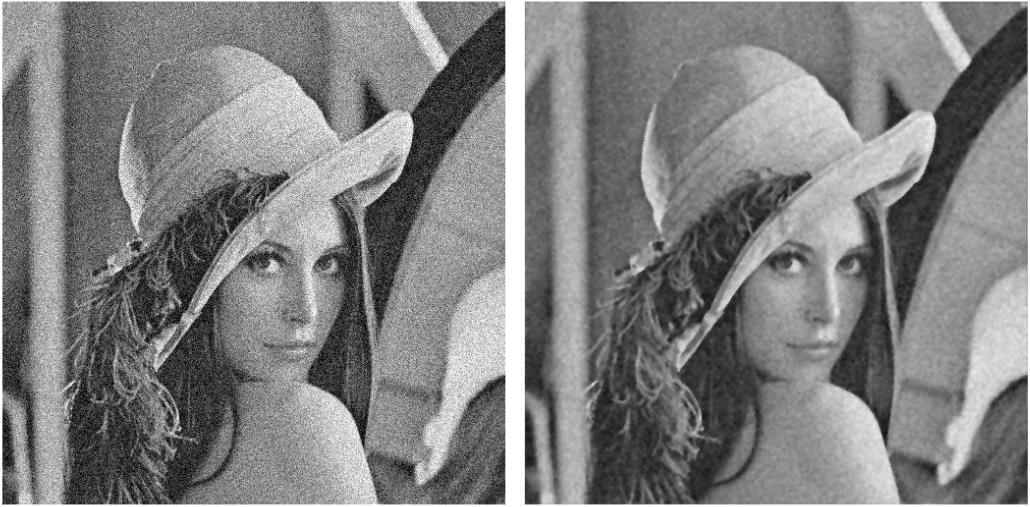
\includegraphics[width=0.6\linewidth] {background/filtering/bilat_filter_eg}
\end{center}
\caption[Example Bilateral Filter]{A bilateral filtering example$\footnotemark$: On the left side a noisy input image on the right its bilateral filtered version.}
\label{fig:bilat_filtering_eg}
\end{figure}
\footnotetext{The shown images have been extracted from: \\ \url{https://www.uni-due.de/mathematik/krommweh/talk_Gemen_Krommweh.pdf}}
The filter replaces the intensity values at each pixel in an image by a weighted average of intensity values from nearby pixels. In our formulation we rely on the Gaussian distributions $G$ for defining the weights. Crucially, the weights depend not only on distances between pixels, but also on the intensity difference. That is why, when iterating through each pixel and adjusting weights to the adjacent pixels accordingly, Sharp edges are preserved. A bilateral filtering example is shown in figure $\ref{fig:bilat_filtering_eg}$.\\ \\
The mathematical definition of this filter is given in equation $\ref{eq:def_bilateral_filter}$. For a given Image $I$ we want to compute its bilateral filtered version by applying the following definition:
\begin{equation}
\begin{aligned}
&\mathcal{F}^{\text{bf}} \{I \} (p) = \frac{1}{W_p} \sum_{q \in \Omega_p} G_{\sigma_s} (\norm{p-q})G_{\sigma_r} (I_p - I_q) I_q \\	
& \text{where } W_p = \sum_{q \in \Omega_p} G_{\sigma_s} (\norm{p-q})G_{\sigma_r} (I_p - I_q)
\end{aligned}
\label{eq:def_bilateral_filter}
\end{equation}
The set $\Omega_p$ contains all neighboring points within the window that are centered at the image point $p$. The scalar $W_p$ denotes the normalization factor of the filter and $I_p$ represents the image intensity at the pixel position $p$. Please notice that the definition of the bilateral filter is given per pixel, i.e. gives an representation of the filtered pixel intensity. \\ \\
The bilateral filter is controlled by the two parameters $\sigma_s$ and $\sigma_r$. The range variance increases $\sigma_r$, the BF becomes closer to the Gaussian blur filter. In other words, the larger $\sigma_r$ the more weight a pixel with a large intensity deviation gets. However, when increasing the spatial variance $\sigma_s$ results in smoothing larger features, i.e more distant pixels get a larger weight and thus influence the result more. Figure $\ref{fig:bfilter_influence_sigmas}$ demonstrates the influence of these parameters.
\begin{figure}[H]
\begin{center}
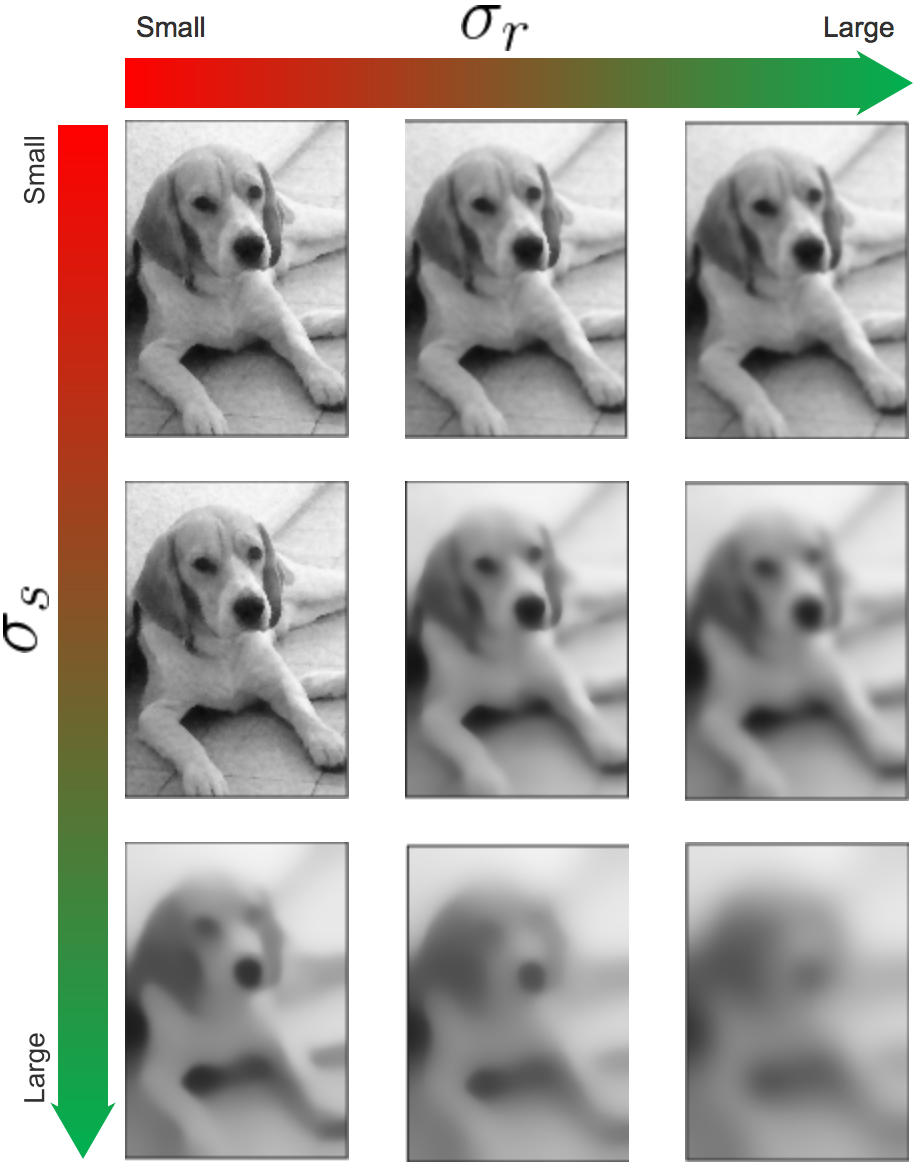
\includegraphics[width=0.6\linewidth] {background/filtering/bilat_filter_sigmas}
\end{center}
\caption[Influence of $\sigma_s$ and $\sigma_r$]{Different filtering results produced by our bilateral filter implementation for varying $\sigma_s$ and $\sigma_r$ values.}
\label{fig:bfilter_influence_sigmas}
\end{figure}

\subsection{Harris Corner Detector}
\label{sec:harris_corner_detector}

% TODO state idea of an edge

Let us consider a grayscale image $I$. We are going to sweep a window $w(x,y)$ (with displacements u in the x direction and v in the right direction) I and will calculate the variation of intensity. Since we are looking for windows with corners, we are looking for windows with a large variation in intensity. Hence, we have to maximize the equation above, specifically the term:
\begin{equation}
	E \left( u, v \right) = \sum_{x,y} w \left( x,y \right) \left[ I(x + u, y + v) - I(x, y) \right]^2
\label{eq:var_intensitiy_def}
\end{equation}
Next, the term $I(x + u, y + v)$ is expressed by the first order taylor series expansion as the follows:
\begin{equation}
	I(x + u, y + v) = I(x,y) + u I_x (x, y) + v I_y (x,y) + \text{h.o.t}
\label{eq:taylor_exp_intensity}
\end{equation}
Next, we put the first order approximation of equation $\ref{eq:taylor_exp_intensity}$ into equation $\ref{eq:var_intensitiy_def}$ to simplify the definition of $E$.
\begin{equation}
\begin{aligned}
E \left( u, v \right) 
&= \sum_{x,y} w \left( x,y \right) \left[ I(x + u, y + v) - I(x, y) \right]^2 \\
&\approx \sum_{x,y} w \left( x,y \right) \left[ I(x,y) + u I_x (x, y) + v I_y (x,y) - I(x, y) \right]^2 \\
&= \sum_{x,y} w \left( x,y \right) \left[ u I_x (x, y) + v I_y (x,y) \right]^2 \\
&= \sum_{x,y} w \left( x,y \right) u^2 I_x^2 + 2 u v I_x I_y v^2 I_y^2 \\
&= \left( u,v \right) \left( \sum_{x,y} w (x,y)
\begin{pmatrix}
I_x^2 & I_x I_y \\
I_x I_y & I_y^2 \\
\end{pmatrix}
\right) \colvec{u}{v}
\end{aligned}
\label{eq:var_intensitiy_developed}
\end{equation}
Let us define the following substitution
\begin{equation}
M = \sum_{x,y} w  (x,y)
\begin{pmatrix}
I_x^2 & I_x I_y \\
I_y^2 & I_x I_y \\
\end{pmatrix}
\label{eq:var_intensity_sub}
\end{equation}
Putting the substitution from equation $\ref{eq:var_intensity_sub}$ into the final form of equation $\ref{eq:var_intensitiy_developed}$ we obtain the final form
\begin{equation}
	E \left( u, v \right) \approx \left( u,v \right) M \colvec{u}{v}
\end{equation}.
A score is calculated for each window, to determine if it can possibly contain a corner:
\begin{equation}
\begin{aligned}
& R = \det(M) - \kappa \left(\text{trace}(M)\right)^2 \\
&\text{where } \det(M) = \lambda_1 \lambda_2 \text{ and } \text{trace}(M) = \lambda_1 + \lambda_2
\end{aligned}
\label{eq:harris_response}
\end{equation}

\section{Camera Model}
explain calibration data
explain pinhole model
explain from scene to camera-space to image-space
mention focal length, principal point
mention how depth could be incooperated
explain intrinsic,extrinsic calibrations
